\documentclass[border=6mm]{standalone}
\usepackage{tikz}
\usetikzlibrary{arrows.meta,calc}

\begin{document}
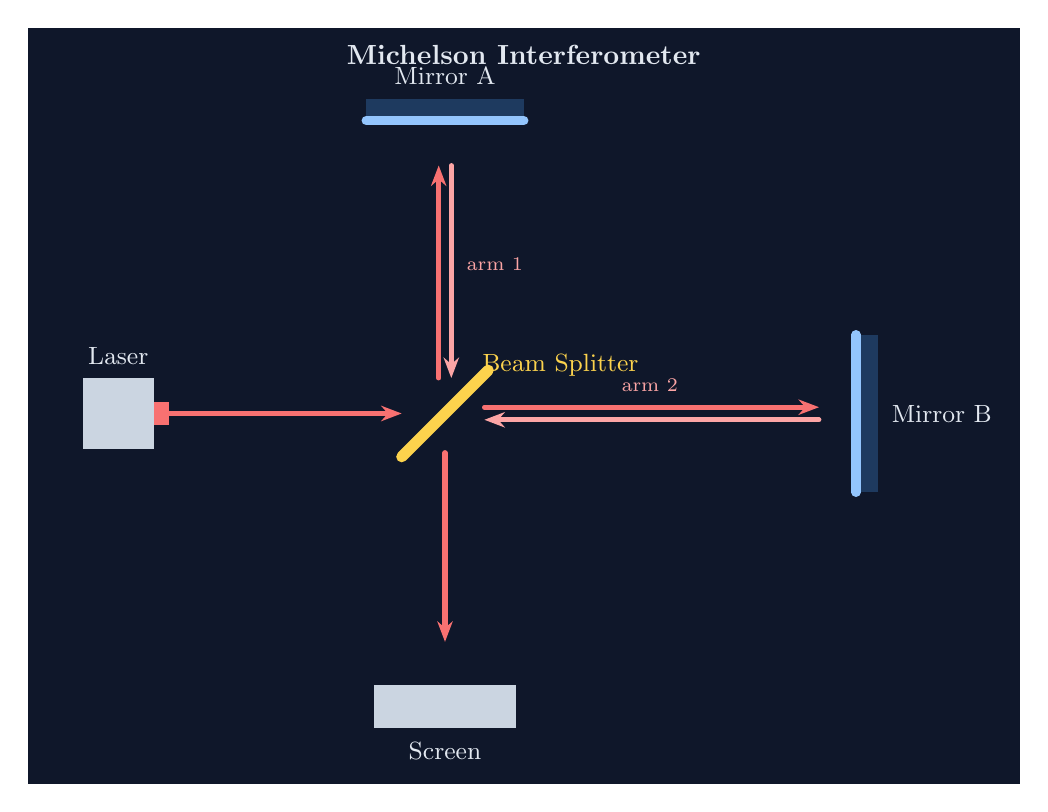
\begin{tikzpicture}[x=1cm,y=1cm,line cap=round,line join=round,
  >={Stealth[length=2.6mm]},font=\sffamily]
  \definecolor{bg}{HTML}{0F172A}
  \definecolor{beam}{HTML}{F87171}
  \definecolor{beam2}{HTML}{FCA5A5}
  \definecolor{mir}{HTML}{93C5FD}
  \definecolor{mirbk}{HTML}{1E3A5F}
  \definecolor{bs}{HTML}{FCD34D}
  \definecolor{dev}{HTML}{CBD5E1}
  \definecolor{lbl}{HTML}{E2E8F0}

  \fill[bg] (-0.3,-0.3) rectangle (12.3,9.3);

  % key points: BS at center (5,4), Laser left (1,4), Mirror B right (10,4),
  % Mirror A top (5,8), Screen bottom (5,0.8)
  \coordinate (BS) at (5,4.4);
  \coordinate (LAS) at (1.2,4.4);
  \coordinate (MB) at (10.2,4.4);
  \coordinate (MA) at (5,8.1);
  \coordinate (SC) at (5,0.9);

  % laser source
  \fill[dev] (0.4,3.95) rectangle (1.3,4.85);
  \fill[beam] (1.3,4.25) rectangle (1.5,4.55);
  \node[lbl,font=\small,anchor=south] at (0.85,4.9) {Laser};

  % beam splitter (45deg plate)
  \draw[bs,line width=0.14cm] ($(BS)+(-0.55,-0.55)$) -- ($(BS)+(0.55,0.55)$);
  \node[bs,font=\small,anchor=south west] at ($(BS)+(0.35,0.35)$) {Beam Splitter};

  % mirror A (top, horizontal)
  \fill[mirbk] (4.0,8.15) rectangle (6.0,8.4);
  \draw[mir,line width=0.12cm] (4.0,8.12) -- (6.0,8.12);
  \node[lbl,font=\small,anchor=south] at (5,8.45) {Mirror A};

  % mirror B (right, vertical)
  \fill[mirbk] (10.25,3.4) rectangle (10.5,5.4);
  \draw[mir,line width=0.12cm] (10.22,3.4) -- (10.22,5.4);
  \node[lbl,font=\small,anchor=west] at (10.55,4.4) {Mirror B};

  % screen / detector (bottom)
  \fill[dev] (4.1,0.4) rectangle (5.9,0.95);
  \node[lbl,font=\small,anchor=north] at (5,0.35) {Screen};

  % beams
  % source -> BS
  \draw[->,beam,line width=0.07cm] (1.5,4.4) -- ($(BS)+(-0.55,0)$);
  % BS -> Mirror A (up) and back (slight offset for visibility)
  \draw[->,beam,line width=0.06cm] ($(BS)+(-0.08,0.45)$) -- ($(MA)+(-0.08,-0.55)$);
  \draw[->,beam2,line width=0.06cm] ($(MA)+(0.08,-0.55)$) -- ($(BS)+(0.08,0.45)$);
  % BS -> Mirror B (right) and back
  \draw[->,beam,line width=0.06cm] ($(BS)+(0.5,0.08)$) -- ($(MB)+(-0.45,0.08)$);
  \draw[->,beam2,line width=0.06cm] ($(MB)+(-0.45,-0.08)$) -- ($(BS)+(0.5,-0.08)$);
  % recombined -> Screen (down)
  \draw[->,beam,line width=0.07cm] ($(BS)+(0,-0.5)$) -- ($(SC)+(0,0.6)$);

  % path labels
  \node[beam2,font=\scriptsize,anchor=west] at (5.15,6.3) {arm 1};
  \node[beam2,font=\scriptsize,anchor=south] at (7.6,4.55) {arm 2};

  \node[lbl,font=\bfseries] at (6,8.95) {Michelson Interferometer};
\end{tikzpicture}
\end{document}
